\documentclass[11pt,a4paper]{article}
\usepackage[margin=2.2cm]{geometry}
\usepackage{graphicx}
\usepackage{booktabs}
\usepackage{amsmath}
\usepackage{siunitx}
\usepackage{xcolor}
\usepackage{caption}
\usepackage{subcaption}
\usepackage{enumitem}
\usepackage[hidelinks]{hyperref}

\graphicspath{{../figures/}}
\setlist{nosep, leftmargin=*}
\captionsetup{font=small}

% Marker for content that depends on phases not finished yet
\newcommand{\pending}[1]{\textcolor{red}{\textbf{[Pending:} #1\textbf{]}}}

\title{ML-Driven PVT-Variation-Aware Leakage Estimation\\[2pt]
       \large Digital VLSI Design --- Course Project Report}
\author{%
  Gaurav Reddy Yerreddi (2024112006) \and
  Neel Rajesh (2024112007) \and
  Monishram Selvaraj (2024112076) \and
  Yogesh Krishna (2024102035)}
\date{}

\begin{document}
\maketitle

\section{Setup}

\begin{table}[!htbp]
\centering
\begin{minipage}[t]{0.52\linewidth}
\centering
\caption{Assignment and simulator.}
\label{tab:setup}
\begin{tabular}{ll}
\toprule
Item & Value \\
\midrule
Model file      & \texttt{32nm\_HP.pm} (PTM BSIM4) \\
Channel length  & $L = L_{\min} = 32$\,nm \\
Nominal VDD     & 0.9\,V \\
Test circuit    & 8-bit parity checker \\
Simulator       & ngspice-47 \\
\bottomrule
\end{tabular}
\end{minipage}\hfill
\begin{minipage}[t]{0.46\linewidth}
\centering
\caption{Nominal process parameters.}
\label{tab:nominal}
\begin{tabular}{lcc}
\toprule
Parameter & NMOS & PMOS \\
\midrule
$v_{th0}$ (V)                  & 0.49396 & $-0.49155$ \\
$t_{oxe}$ (nm)                 & 1.15 & 1.20 \\
$n_{dep}$ (cm$^{-3}$)          & $4.12\times10^{18}$ & $3.07\times10^{18}$ \\
$u_0$ (m$^2$/V\,s)             & 0.050 & 0.014 \\
$x_j$ (nm)                     & 10 & 10 \\
\bottomrule
\end{tabular}
\end{minipage}
\end{table}

The nominal values in Table~\ref{tab:nominal} are read from the model card. Models were trained
with Python 3.11, PyTorch 2.15 and scikit-learn 1.9 on CPU. All scripts read the assignment, sampling ranges and seeds from a single \texttt{config.yaml},
and run in numeric order.

\section{Data generation}

\subsection{Sampling}
For each of the four cases (NMOS ON, NMOS OFF, PMOS ON, PMOS OFF), 10,000 samples were drawn
independently (seed 2026, one random stream per case), following Section~4 of the project spec:
\begin{itemize}
  \item $V_{DD} \sim U(0.81, 0.99)$\,V, drawn first; then $V_d, V_s \sim U(0, V_{DD})$;
  \item $W \sim U(1, 8)\cdot L_{\min}$; $T \sim U(-40, 125)$\,\si{\celsius};
  \item $v_{th0}, t_{oxe}, n_{dep}, u_0, x_j$ each $= \text{nominal}\times U(0.9, 1.1)$, drawn separately for NMOS and PMOS;
  \item $V_g, V_b$ fixed by the case (NMOS ON: $V_{DD}, 0$; NMOS OFF: $0, 0$; PMOS ON: $0, V_{DD}$; PMOS OFF: $V_{DD}, V_{DD}$).
\end{itemize}
Each dataset is stored as one CSV with columns
\texttt{vdd, temp, w, vd, vs, vg, vb, vth0, toxe, ndep, u0, xj, id, ig, is, ib} (SI units).

\subsection{Netlists}
Each case has a hand-written single-transistor netlist (\texttt{netlists/transistor/<case>.cir})
that runs on its own with \texttt{ngspice -b}. Every terminal has its own DC voltage source, and
each netlist contains the required
\texttt{.options gmin=1e-18 abstol=1e-18 reltol=1e-6 vntol=1e-9}.
The generation script replaces the \texttt{.param} values with each sample and runs ngspice
once per sample (about 2 minutes for all 40,000 runs, 8 parallel processes). Further details:
\begin{itemize}
  \item \textbf{Process parameters} are applied with \texttt{altermod}, one line per parameter:
        a multi-parameter \texttt{altermod} line in ngspice silently applies only the first one.
        A sensitivity test confirmed that all five parameters reach the simulator.
  \item \textbf{Junction geometry:} $AD = AS = W L_{\mathrm{diff}}$, $PD = PS = 2(W + L_{\mathrm{diff}})$ with
        $L_{\mathrm{diff}} = 2L_{\min}$ (as in the TA example netlist). Only $I_b$ depends on it.
  \item \textbf{Sign convention:} every stored current flows \emph{into} the device terminal
        ($I = -\,\texttt{i(Vsource)}$). \texttt{set numdgt=12} is used so that printed currents
        are not rounded to 6 digits.
\end{itemize}

\subsection{Train / validation / test split}
Each dataset was split 70/15/15 (7,000 / 1,500 / 1,500 rows) with a fixed seed (42). The split
is stored as a file per case and shared by all four model types, so every model is trained,
tuned and tested on exactly the same rows. Tuning used the validation set only; the test set is
used only for the chosen model.

\subsection{Data check}
\paragraph{Kirchhoff check.} Table~\ref{tab:kcl} lists $|I_d + I_g + I_s + I_b|$ per case.
The residual of about \SI{1e-16}{A} comes from the gate and substrate resistance networks
enabled in the PTM card (\texttt{rgatemod=1}, \texttt{rbodymod=1}); with both switched off the
residual drops to \SI{1e-31}{A}. The model card was used unmodified. The practical consequence
is a simulator noise floor: currents below about \SI{1e-15}{A} are not reproducible between
equivalent simulations. This affects mainly PMOS OFF $I_g$ (62\,\% of rows), PMOS OFF and NMOS OFF
$I_b$ (54\,\%), and about 20\,\% of PMOS OFF $I_d/I_s$.

\begin{table}[!htbp]
\centering
\caption{Kirchhoff check: $|I_d+I_g+I_s+I_b|$ over the 10,000 samples of each case.}
\label{tab:kcl}
\begin{tabular}{lcc}
\toprule
Case & Median (A) & Max (A) \\
\midrule
NMOS ON  & \num{9.1e-17} & \num{1.2e-15} \\
NMOS OFF & \num{2.0e-23} & \num{5.1e-20} \\
PMOS ON  & \num{3.0e-17} & \num{6.0e-16} \\
PMOS OFF & \num{7.7e-17} & \num{1.0e-15} \\
\bottomrule
\end{tabular}
\end{table}

\paragraph{Trend plots.} Figure~\ref{fig:trends} shows the raw dataset values. OFF current
($|I_d|$ of the OFF datasets) rises by several decades from $-40$ to \SI{125}{\celsius}
(subthreshold slope and $V_{th}$ fall with temperature). Gate current falls steeply with $t_{oxe}$,
as expected for direct tunnelling. OFF current also falls with $|v_{th0}|$, but this trend is
weaker in the raw scatter: a $\pm10\,\%$ change in $v_{th0}$ moves $I_{\mathrm{off}}$ less than the spread
caused by the other random inputs ($T$, $W$, $V_d$, $V_s$). PMOS ON gate current sits lower than
a nominal sweep would suggest because the random $V_s$ often gives a small $|V_{gs}|$.

\begin{figure}[!htbp]
\centering
\begin{subfigure}{0.32\linewidth}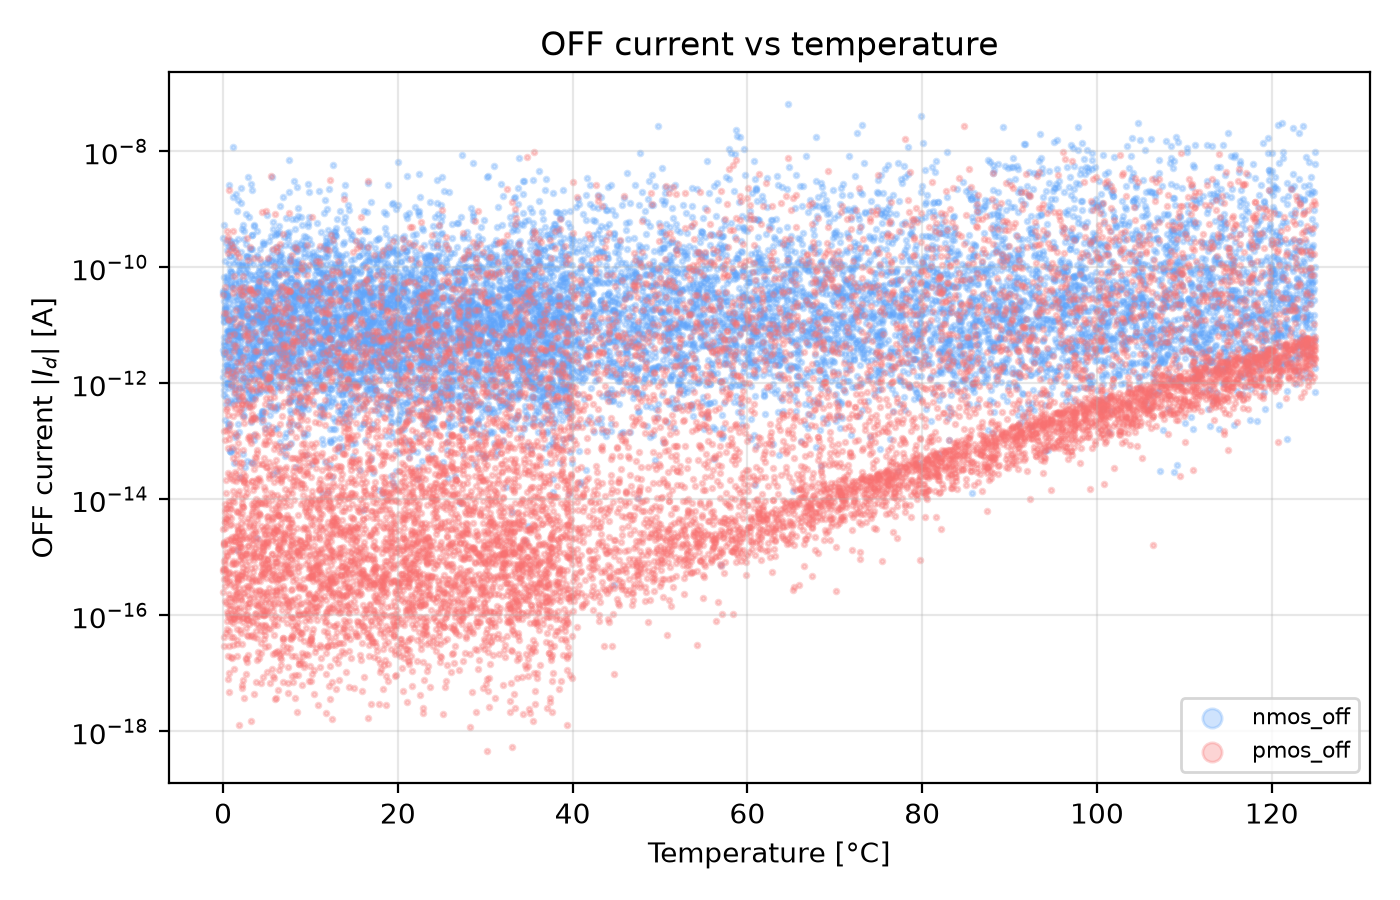
\includegraphics[width=\linewidth]{trend_ioff_vs_temp.png}\caption{$I_{\mathrm{off}}$ vs $T$}\end{subfigure}
\begin{subfigure}{0.32\linewidth}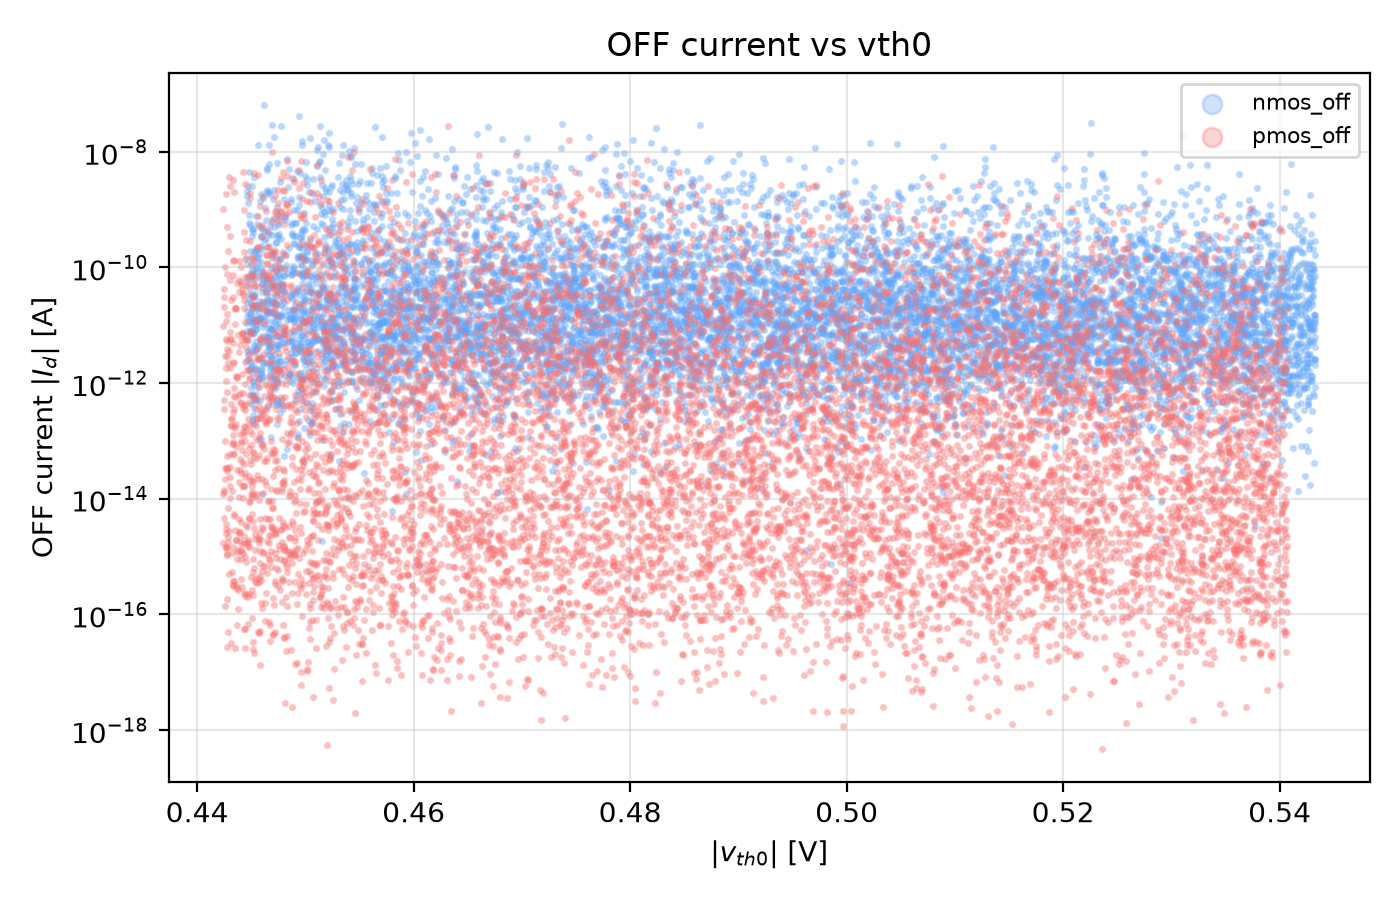
\includegraphics[width=\linewidth]{trend_ioff_vs_vth0.png}\caption{$I_{\mathrm{off}}$ vs $|v_{th0}|$}\end{subfigure}
\begin{subfigure}{0.32\linewidth}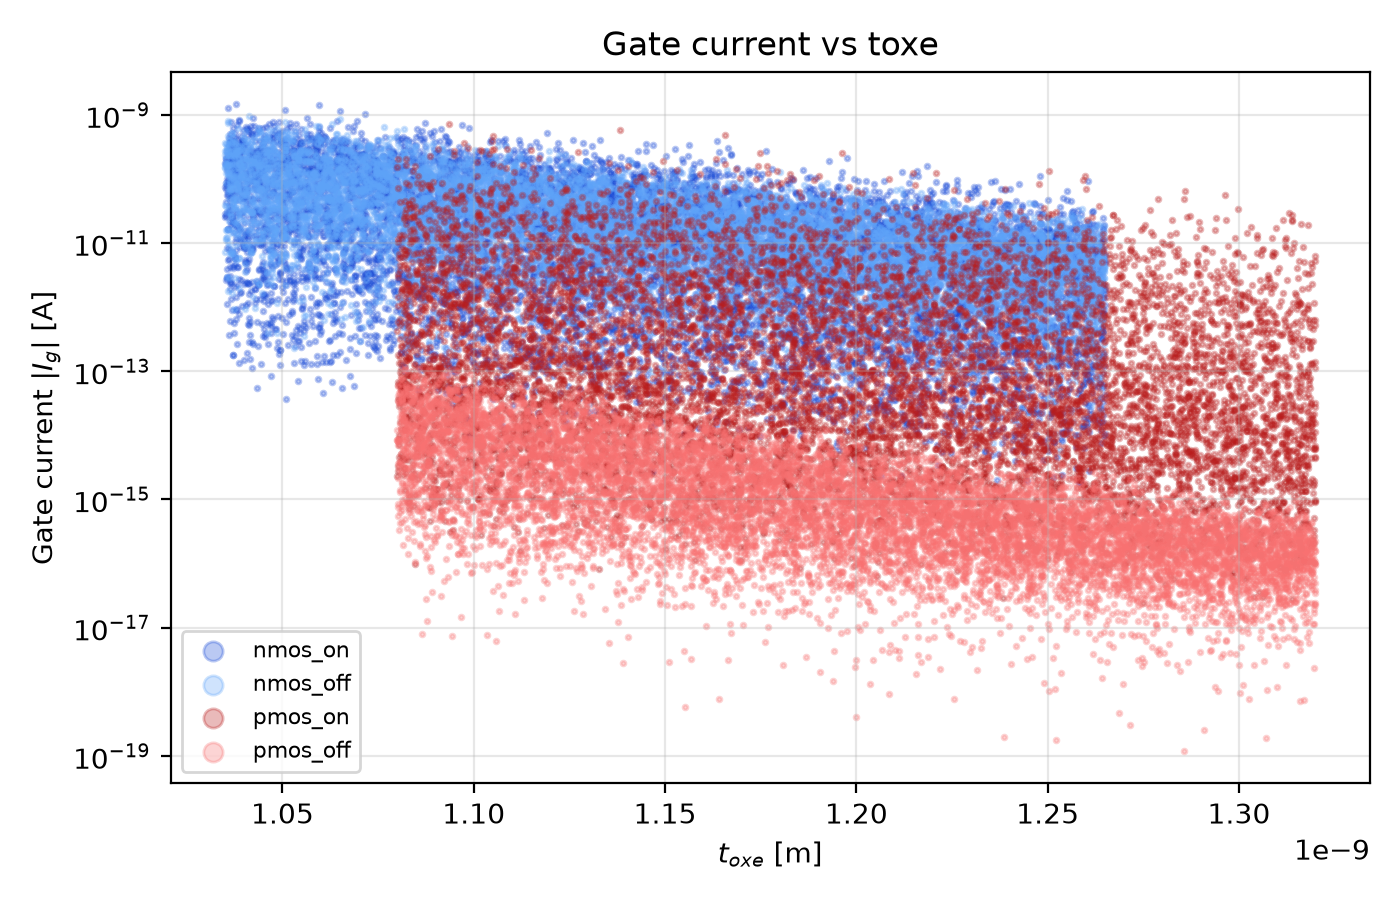
\includegraphics[width=\linewidth]{trend_ig_vs_toxe.png}\caption{$|I_g|$ vs $t_{oxe}$}\end{subfigure}
\caption{Data-check trend plots (NMOS and PMOS in different colours).}
\label{fig:trends}
\end{figure}

\section{Models}

\subsection{Common preprocessing and metrics}
All four model types use the same conventions:
\begin{itemize}
  \item \textbf{Target scale:} each current is predicted as $\operatorname{asinh}(I / \SI{1e-18}{A})$
        instead of $I$. Currents span 6--13 decades and many change sign (about half of $I_d/I_s$
        in the ON cases are negative), so $\log|I|$ would lose the sign. Above about \SI{1e-17}{A},
        $\operatorname{asinh}(I/I_0) \approx \operatorname{sign}(I)\ln(2|I|/I_0)$, i.e.\ a
        sign-preserving log.
  \item \textbf{Error:} relative error $|I_{\mathrm{pred}}-I_{\mathrm{SPICE}}|/|I_{\mathrm{SPICE}}|\times100\,\%$, reported as
        the median and 95th percentile per current, on all rows (noise-floor currents included).
  \item \textbf{$R^2$} is computed on the $\operatorname{asinh}(I/\SI{1e-18}{A})$ scale. On a log-like
        scale even mediocre fits score above 0.99, so models are ranked on median and p95 error;
        $R^2$ is a secondary check.
\end{itemize}

\subsection{Model types}
\paragraph{MLP (PyTorch).} Inputs: the 12 CSV inputs plus 4 derived features
($V_d-V_s$, $V_g-V_s$, $V_b-V_s$, $1/T$ in K), standardised on the training set. Outputs: the four
asinh-scaled currents, each standardised. Fully connected network with SiLU activations, L1 loss,
AdamW, one-cycle learning-rate schedule (peak $3\times10^{-3}$), batch 256, seed 42.
ON cases: $128\times3$ layers, 6,000 epochs, no weight decay; OFF cases: $256\times4$ layers,
3,000 epochs, weight decay $10^{-3}$.
These settings came from a two-round search on the validation set (Appendix~\ref{app:mlp}):
L1 loss clearly beat MSE and Huber, SiLU beat tanh and GELU, and a peak LR of 0.01 was worse.
A first scikit-learn \texttt{MLPRegressor} underfit (6--7\,\% median error at best; it had no
LR schedule and stopped early); the move to PyTorch with an LR schedule, L1 loss and per-output
scaling brought the error below 1\,\%.

\paragraph{Model type 2.} \pending{teammate's model, main hyperparameters, preprocessing}

\paragraph{Model type 3.} \pending{teammate's model, main hyperparameters, preprocessing}

\paragraph{Model type 4.} \pending{teammate's model, main hyperparameters, preprocessing}

\subsection{Model comparison (validation set)}
Table~\ref{tab:cmp} gives the median error, p95 error and $R^2$ for each current, in the order
$I_d / I_g / I_s / I_b$.

\begin{table}[!htbp]
\centering
\footnotesize
\caption{Validation-set comparison (4 model types $\times$ 4 cases). Errors in \%;
$R^2$ on the $\operatorname{asinh}(I/\SI{1e-18}{A})$ scale. Each cell: $I_d / I_g / I_s / I_b$.}
\label{tab:cmp}
\setlength{\tabcolsep}{4pt}
\begin{tabular}{llccc}
\toprule
Model & Case & Median error (\%) & p95 error (\%) & $R^2$ \\
\midrule
MLP & NMOS ON  & 1.02 / 0.33 / 1.03 / 0.47 & 10.3 / 3.2 / 10.6 / 2.7 & .9918 / .9999 / .9916 / 1.000 \\
    & NMOS OFF & 0.77 / 0.16 / 0.82 / 0.51 & 15.7 / 1.3 / 20.9 / 4.6 & .9878 / 1.000 / .9817 / 1.000 \\
    & PMOS ON  & 1.03 / 0.30 / 1.03 / 0.48 & 15.4 / 1.5 / 14.6 / 4.3 & .9881 / 1.000 / .9888 / .9998 \\
    & PMOS OFF & 7.88 / 14.99 / 7.82 / 17.29 & 63.5 / 226.5 / 78.8 / 243.3 & .9847 / .3980 / .9865 / .8186 \\
\midrule
Type 2 & all & \multicolumn{3}{c}{\pending{results}} \\
Type 3 & all & \multicolumn{3}{c}{\pending{results}} \\
Type 4 & all & \multicolumn{3}{c}{\pending{results}} \\
\bottomrule
\end{tabular}
\end{table}

\subsection{Final choice and test-set results}
\pending{chosen model per case with the reason, test-set median / p95 error, predicted-vs-SPICE
plot per case.}

\section{Gate results}
\pending{Phases 4--5: gate results table (18 cases: SPICE median, ML median, bias, median error,
p95 error), gate parity plot on log axes, and comment on the most and least accurate gates and
input combinations.}

\section{Test-circuit results}
The 8-bit parity checker is built only from gates that have ML models: each XOR2 is four NAND2
gates, and the 7 XOR2 gates form a tree over the 8 inputs.
\pending{Phase 6: test-circuit metrics table, parity plot, and comparison with gate-level accuracy.}

\section{Error analysis}
At the transistor level (MLP, validation set):
\begin{itemize}
  \item \textbf{PMOS OFF is the hardest case} (12\,\% mean median error vs 0.6--0.7\,\% for the
        others), driven by $I_g$ and $I_b$. Most of these currents are below \SI{1e-15}{A}, i.e.\
        at the simulator noise floor found in the Kirchhoff check, so the targets themselves are
        not reproducible. The network memorises this noise (training error near 0\,\%) and cannot
        generalise it; the error is limited by the data, not the model.
  \item \textbf{$I_d$ and $I_s$ have the largest p95 errors} in every case (10--21\,\% in the
        non-PMOS-OFF cases). They occur where $V_d \approx V_s$: the channel current passes
        through zero and changes sign, so the relative error of a small absolute error is large.
  \item $I_g$ and $I_b$ in NMOS ON, NMOS OFF and PMOS ON are the most accurate currents
        (median $\le 0.5\,\%$), as they vary smoothly with the inputs.
\end{itemize}
\pending{gate- and circuit-level error analysis: worst gates, input combinations and corner
conditions (temperature, $v_{th0}$).}

\section{Limitations and improvements}
\begin{itemize}
  \item \textbf{Simulator noise floor.} Currents below \SI{1e-15}{A} are not reproducible with
        the unmodified card, which caps the accuracy for PMOS OFF $I_g/I_b$. These currents are
        negligible in a gate sum, so their effect on gate leakage should be small.
  \item \textbf{Sampling near $V_d \approx V_s$.} Uniform sampling places few points where the
        channel current changes sign; denser sampling there would reduce the $I_d/I_s$ tail error.
  \item \textbf{Ensembling.} Averaging five MLPs trained with seeds 42--46 roughly halved the median
        error in our tests (e.g.\ NMOS ON 0.71\,\% $\to$ 0.40\,\%, PMOS OFF 12.0\,\% $\to$ 8.8\,\%)
        at five times the training cost.
  \item \textbf{Hyperparameter search} was done manually in two rounds and is not reproduced by
        the final script, which uses the fixed settings found.
  \item \textbf{Hierarchical assumptions} (exact 0/VDD gate inputs, no loading between gates) will
        add error at the circuit level. \pending{quantify after Phase 6.}
\end{itemize}

\appendix
\section{MLP hyperparameter search}
\label{app:mlp}
Values are the validation mean of the four median errors.

\begin{table}[!htbp]
\centering
\small
\caption{Round 1 (base: $128\times3$, SiLU, MSE, peak LR $3\times10^{-3}$, batch 256, 3,000 epochs; one change per row).}
\begin{tabular}{llcc}
\toprule
\# & Change from base & NMOS ON & PMOS OFF \\
\midrule
1 & none                      & 1.54\,\% & 24.20\,\% \\
2 & $256\times4$              & 2.09\,\% & 21.51\,\% \\
3 & L1 loss                   & \textbf{0.87\,\%} & 18.32\,\% \\
4 & Huber loss                & 1.35\,\% & 20.21\,\% \\
5 & $256\times4$ + L1 loss    & 1.10\,\% & \textbf{12.56\,\%} \\
6 & tanh                      & 2.31\,\% & 56.25\,\% \\
7 & $256\times4$ + GELU       & 1.88\,\% & 25.00\,\% \\
8 & $256\times4$ + peak LR 0.01 & 2.84\,\% & 30.05\,\% \\
\bottomrule
\end{tabular}
\end{table}

\begin{table}[!htbp]
\centering
\small
\caption{Round 2 (all L1 loss, SiLU, peak LR $3\times10^{-3}$).}
\begin{tabular}{llcccc}
\toprule
 & Setting & NMOS ON & NMOS OFF & PMOS ON & PMOS OFF \\
\midrule
A & $128\times3$, 3,000 epochs          & 0.87\,\% & 0.81\,\% & 0.91\,\% & 18.32\,\% \\
B & $256\times4$, 3,000 epochs          & 1.10\,\% & 0.60\,\% & 0.92\,\% & 12.56\,\% \\
C & $128\times3$, 6,000 epochs          & \textbf{0.71\,\%} & 0.58\,\% & \textbf{0.71\,\%} & 15.66\,\% \\
D & $256\times4$, weight decay $10^{-3}$ & 1.00\,\% & \textbf{0.57\,\%} & 0.90\,\% & \textbf{12.00\,\%} \\
E & $128\times3$, batch 128             & 0.72\,\% & 0.62\,\% & 0.73\,\% & 14.37\,\% \\
\bottomrule
\end{tabular}
\end{table}

\end{document}
